% 第三章 图表、公式格式
\thesischapterpage{3\quad 图表、公式格式}

\section{图表、公式格式}

\subsection{图表格式}
\thesisbodyfont
本章主要展示图、表和公式的排版方式。正文中引用图表时，应先在文字中说明图表含义，再给出图表内容。图题一般位于图下方，表题一般位于表上方。

\begin{figure}[htb]
  \centering
  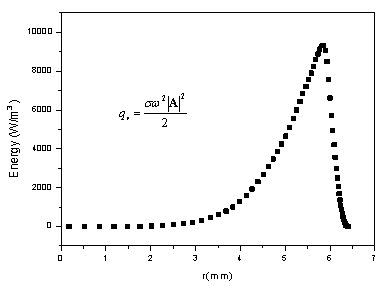
\includegraphics[width=0.95\textwidth]{assets/figures/chapter3/fig2.PNG}
  \caption{内热源沿径向的分布}
  \label{fig:radial_heat_source}
\end{figure}

\begin{table}[htbp]
\centering
\caption{高频感应加热的基本参数}
\label{tab:heating_parameters}
\small
\begin{tabular}{c c c c}
\toprule
感应频率 & 感应发生器功率 & 工件移动速度 & 感应圈与零件间隙\\
（KHz） & ($\% \times$80Kw) & (mm/min) & (mm)\\
\midrule
250 & 88 & 5900 & 1.65\\
250 & 88 & 5900 & 1.65\\
250 & 88 & 5900 & 1.65\\
250 & 88 & 5900 & 1.65\\
\bottomrule
\end{tabular}
\end{table}

\begin{table}[htbp]
\centering
\captionsetup{singlelinecheck=off}
\caption*{续表3.1}
\small
\begin{tabular}{c c c c}
\toprule
感应频率 & 感应发生器功率 & 工件移动速度 & 感应圈与零件间隙\\
（KHz） & ($\% \times$80Kw) & (mm/min) & (mm)\\
\midrule
250 & 88 & 5900 & 1.65\\
250 & 88 & 5900 & 1.65\\
\bottomrule
\end{tabular}
\end{table}

\subsection{公式格式}
\thesisbodyfont
公式应按章节编号，重要公式应在正文中解释变量含义。示例如下：

\begin{eqnarray}
\frac{1}{\mu} \nabla^2A - j \omega \sigma A -\nabla(\frac{1}{\mu}) \times(\nabla \times A)+J_0=0
\end{eqnarray}

\subsection{算法格式}
\thesisbodyfont
计算机相关论文可根据需要使用算法环境。以下示例用于验证算法标题、编号和输入输出关键词的格式。

\begin{algorithm}[htbp]
\caption{模板算法示例}
\KwIn{输入数据 $X$}
\KwOut{计算结果 $Y$}
\KwInit{$Y \leftarrow 0$}
\ForEach{$x \in X$}{
  更新中间结果 $Y$\;
}
\KwReturn{$Y$}
\end{algorithm}

\subsection{本章小结}
\thesisbodyfont
本章展示了图、表、续表、公式和算法的基本排版效果。
